% 5-minute talk — see slideshow_plans.md. Built with the existing TinyTeX/latexmk
% toolchain (beamer installed via tlmgr). Numbers come from the script-generated
% macros (\input paper_macros.tex); figures are the generated PNGs. Build:
%   latexmk -pdf talk.tex
\documentclass[aspectratio=169]{beamer}
\usetheme{Madrid}
\usepackage{graphicx}
\usepackage{booktabs}
\graphicspath{{../results/counter_decode/self_calibration/}}
% AUTO-GENERATED by scripts/build_paper_macros.py -- do not edit by hand.
% Data sources: results/counter_decode/{tables,sliding_filter_mixed,
%   entropy_probe,belief_sweep,belief_invariance}/*.json and
%   results/tables/{blacklist,topk}_summary*.json ; plus the
%   per-experiment macro files calibration_baseline/macros.tex and
%   natural_text/macros.tex (digit-in-name sanitised to a word).

\newcommand{\binvCeExplode}{19.44}
\newcommand{\binvCeFloor}{3.60}
\newcommand{\binvSigmaZero}{0.2}
\newcommand{\binvVarCap}{0.07}
\newcommand{\binvVarFloor}{0.017}
\newcommand{\blRankOneDeltaP}{-0.019}
\newcommand{\blRankOneTvc}{-0.016}
\newcommand{\blRankOneTvcHi}{-0.013}
\newcommand{\blRankOneTvcLo}{-0.019}
\newcommand{\bsweepBestBadness}{0.011}
\newcommand{\calConsistencyGapWP}{-0.765}
\newcommand{\calConsistencyGapWT}{-0.938}
\newcommand{\calLength}{256}
\newcommand{\calLogBetaMLEWP}{-0.036}
\newcommand{\calLogBetaMLEWT}{+0.000}
\newcommand{\calLogBetaStreamMedWP}{-0.314}
\newcommand{\calLogBetaStreamMedWT}{-0.059}
\newcommand{\calLogBetaStreamPooledWP}{-0.802}
\newcommand{\calLogBetaStreamPooledWT}{-0.937}
\newcommand{\calNcal}{60}
\newcommand{\calNllMLEWP}{2.9992}
\newcommand{\calNllMLEWT}{1.9724}
\newcommand{\calNllOneWP}{3.0029}
\newcommand{\calNllOneWT}{1.9724}
\newcommand{\calNtest}{60}
\newcommand{\calSigmaZero}{0.5}
\newcommand{\calTestDeltaLogPPLWPTOne}{+0.0000}
\newcommand{\calTestDeltaLogPPLWPWPMLE}{-0.0011}
\newcommand{\calTestDeltaLogPPLWPWPstreammed}{+0.2522}
\newcommand{\calTestDeltaLogPPLWPWPstreampooled}{+2.0103}
\newcommand{\calTestDeltaLogPPLWPWTMLE}{+0.0001}
\newcommand{\calTestDeltaLogPPLWTTOne}{+0.0000}
\newcommand{\calTestDeltaLogPPLWTWPMLE}{+0.0014}
\newcommand{\calTestDeltaLogPPLWTWTMLE}{+0.0000}
\newcommand{\calTestDeltaLogPPLWTWTstreammed}{+0.0048}
\newcommand{\calTestDeltaLogPPLWTWTstreampooled}{+2.6543}
\newcommand{\calTestPPLWPTOne}{19.553}
\newcommand{\calTestPPLWPWPMLE}{19.485}
\newcommand{\calTestPPLWPWPstreammed}{24.989}
\newcommand{\calTestPPLWPWPstreampooled}{143.398}
\newcommand{\calTestPPLWPWTMLE}{19.555}
\newcommand{\calTestPPLWTTOne}{7.353}
\newcommand{\calTestPPLWTWPMLE}{7.361}
\newcommand{\calTestPPLWTWTMLE}{7.353}
\newcommand{\calTestPPLWTWTstreammed}{7.385}
\newcommand{\calTestPPLWTWTstreampooled}{105.248}
\newcommand{\calTestPValWPTOne}{1}
\newcommand{\calTestPValWPWPMLE}{0.347}
\newcommand{\calTestPValWPWPstreammed}{2.02e-34}
\newcommand{\calTestPValWPWPstreampooled}{1.29e-64}
\newcommand{\calTestPValWPWTMLE}{0.000203}
\newcommand{\calTestPValWTTOne}{1}
\newcommand{\calTestPValWTWPMLE}{0.0245}
\newcommand{\calTestPValWTWTMLE}{0.0684}
\newcommand{\calTestPValWTWTstreammed}{6.31e-06}
\newcommand{\calTestPValWTWTstreampooled}{1.15e-79}
\newcommand{\calTestTStatWPTOne}{+0.00}
\newcommand{\calTestTStatWPWPMLE}{-0.95}
\newcommand{\calTestTStatWPWPstreammed}{+26.46}
\newcommand{\calTestTStatWPWPstreampooled}{+89.13}
\newcommand{\calTestTStatWPWTMLE}{+3.96}
\newcommand{\calTestTStatWTTOne}{+0.00}
\newcommand{\calTestTStatWTWPMLE}{+2.31}
\newcommand{\calTestTStatWTWTMLE}{+1.86}
\newcommand{\calTestTStatWTWTstreammed}{+4.96}
\newcommand{\calTestTStatWTWTstreampooled}{+160.77}
\newcommand{\calU}{236}
\newcommand{\calWarmup}{20}
\newcommand{\expbEntropyGap}{1.34}
\newcommand{\expbGenreGap}{+0.054}
\newcommand{\expbHwiki}{1.686}
\newcommand{\expbHwp}{3.024}
\newcommand{\expbSaturated}{-0.46}
\newcommand{\expcLateHalf}{9.216}
\newcommand{\expcLateTwo}{1.172}
\newcommand{\expcSpread}{8.04}
\newcommand{\expcSpreadT}{+69.7}
\newcommand{\expcSwapPostFifty}{8.91}
\newcommand{\expcSwapPre}{8.56}
\newcommand{\expcSwitchStep}{80}
\newcommand{\fzeroEuncoHalf}{4.74}
\newcommand{\fzeroLogbhatHalf}{-4.74}
\newcommand{\fzeroMaxPcorrHalf}{0.579}
\newcommand{\fzeroMaxPuncoHalf}{0.001}
\newcommand{\fzeroRfinal}{0.15}
\newcommand{\logBetaFinalIqrHighWPNat}{-0.089}
\newcommand{\logBetaFinalIqrHighWPSelf}{+0.127}
\newcommand{\logBetaFinalIqrHighWikiNat}{+0.162}
\newcommand{\logBetaFinalIqrHighWikiSelf}{+0.052}
\newcommand{\logBetaFinalIqrLowWPNat}{-0.702}
\newcommand{\logBetaFinalIqrLowWPSelf}{-0.255}
\newcommand{\logBetaFinalIqrLowWikiNat}{-0.475}
\newcommand{\logBetaFinalIqrLowWikiSelf}{-0.334}
\newcommand{\logBetaFinalMedWPNat}{-0.236}
\newcommand{\logBetaFinalMedWPSelf}{-0.052}
\newcommand{\logBetaFinalMedWikiNat}{-0.065}
\newcommand{\logBetaFinalMedWikiSelf}{-0.070}
\newcommand{\logBetaFinalSeWPNat}{0.074}
\newcommand{\logBetaFinalSeWPSelf}{0.054}
\newcommand{\logBetaFinalSeWikiNat}{0.093}
\newcommand{\logBetaFinalSeWikiSelf}{0.068}
\newcommand{\logBetaFinalTWPNat}{-3.19}
\newcommand{\logBetaFinalTWPSelf}{-0.96}
\newcommand{\logBetaFinalTWikiNat}{-0.70}
\newcommand{\logBetaFinalTWikiSelf}{-1.03}
\newcommand{\logBetaFinalTrimMedWPNat}{-0.236}
\newcommand{\logBetaFinalTrimMedWPSelf}{-0.052}
\newcommand{\logBetaFinalTrimMedWikiNat}{-0.065}
\newcommand{\logBetaFinalTrimMedWikiSelf}{-0.070}
\newcommand{\meanEntropyWPNat}{2.847}
\newcommand{\meanEntropyWPSelf}{2.939}
\newcommand{\meanEntropyWikiNat}{1.983}
\newcommand{\meanEntropyWikiSelf}{2.691}
\newcommand{\nPassagesWPNat}{64}
\newcommand{\nPassagesWPSelf}{64}
\newcommand{\nPassagesWikiNat}{64}
\newcommand{\nPassagesWikiSelf}{64}
\newcommand{\pairedMeanDiffWP}{-0.304}
\newcommand{\pairedMeanDiffWiki}{-0.050}
\newcommand{\pairedMedianDiffWP}{-0.328}
\newcommand{\pairedMedianDiffWiki}{-0.058}
\newcommand{\pairedSeDiffWP}{0.080}
\newcommand{\pairedSeDiffWiki}{0.096}
\newcommand{\pairedTStatWP}{-3.80}
\newcommand{\pairedTStatWiki}{-0.52}
\newcommand{\priorMode}{-0.125}
\newcommand{\sigmaZero}{0.5}
\newcommand{\tkDeltaKfive}{+0.170}
\newcommand{\tkDeltaKthree}{+0.475}
\newcommand{\totalFisherWPNat}{1017}
\newcommand{\totalFisherWPSelf}{1019}
\newcommand{\totalFisherWikiNat}{751}
\newcommand{\totalFisherWikiSelf}{1041}
   % script-sourced numbers; never hand-typed

\title[LLMs figure out their decoder]{Modeling and Calibrating:\\ LLMs Figure out their Decoding Process}
\author{Matthew Khoriaty}
\institute{Reliable ML with Unreliable Black Boxes}
\date{\today}

\begin{document}

\frame{\titlepage}

% ---------------------------------------------------------------------------
\begin{frame}{The question}
  \begin{itemize}
    \item An autoregressive LM is trained to \emph{predict} text --- so when it
      \emph{generates}, it has an incentive to model its own \textbf{decoder}
      (temperature, top-$k$, \dots).
    \item Two questions: \textbf{(a)} does it? \quad \textbf{(b)} can we use that to
      predict better?
  \end{itemize}
  \vfill
  \begin{block}{}
    \centering Can a model read the \emph{temperature} of the text in front of it,
    and recalibrate itself?
  \end{block}
\end{frame}

% ---------------------------------------------------------------------------
\begin{frame}{The tool: a streaming Bayesian filter on $\log\beta$}
  \begin{itemize}
    \item A Laplace filter maintains a posterior on $\eta=\log\beta$
      (inverse-temperature), updated \emph{per token} from the prefix ---
      online, causal, training-free. $\hat\beta_t$ depends only on $x_{<t}$.
    \item Each token is a Newton / Fisher-scoring step on
      $P(x\mid\eta)=\mathrm{softmax}(e^{\eta}\ell)[x]$.
    \item \textbf{Fix (this work):} the production filter linearises at $\beta=1$ and is
      \emph{inconsistent}. The \emph{faithful} filter re-linearises at the running
      $\hat\beta$, with the correct $\beta,\beta^{2}$ chain-rule terms.
  \end{itemize}
\end{frame}

% ---------------------------------------------------------------------------
\begin{frame}{Two honest negatives (clearing the ground)}
  \begin{itemize}
    \item \textbf{Closed-loop correction self-neutralises.} Feeding $\hat\beta$ back into
      the sampler drives $\beta_{\mathrm{dec}}\to1$ --- the temperature is quietly thrown
      away. Confirmed across exact-grid filters (not an approximation artifact).
    \item \textbf{Real creative writing is already calibrated.} The best single
      temperature gives a non-significant fraction-of-a-nat gain --- nothing to fix.
  \end{itemize}
  \vfill
  \centering\emph{So: to show self-calibration works, test where the temperature is
  \textbf{known} and there is something to recover.}
\end{frame}

% ---------------------------------------------------------------------------
\begin{frame}{Claim 1: recovering a \emph{known} decoder temperature}
  \footnotesize Generate Qwen-2.5-3B self-text at a known $\beta=1/T$
  ($\scNseq$ sequences per $T$); run the filter causally over it.
  \begin{columns}[T]
    \column{0.52\textwidth}
      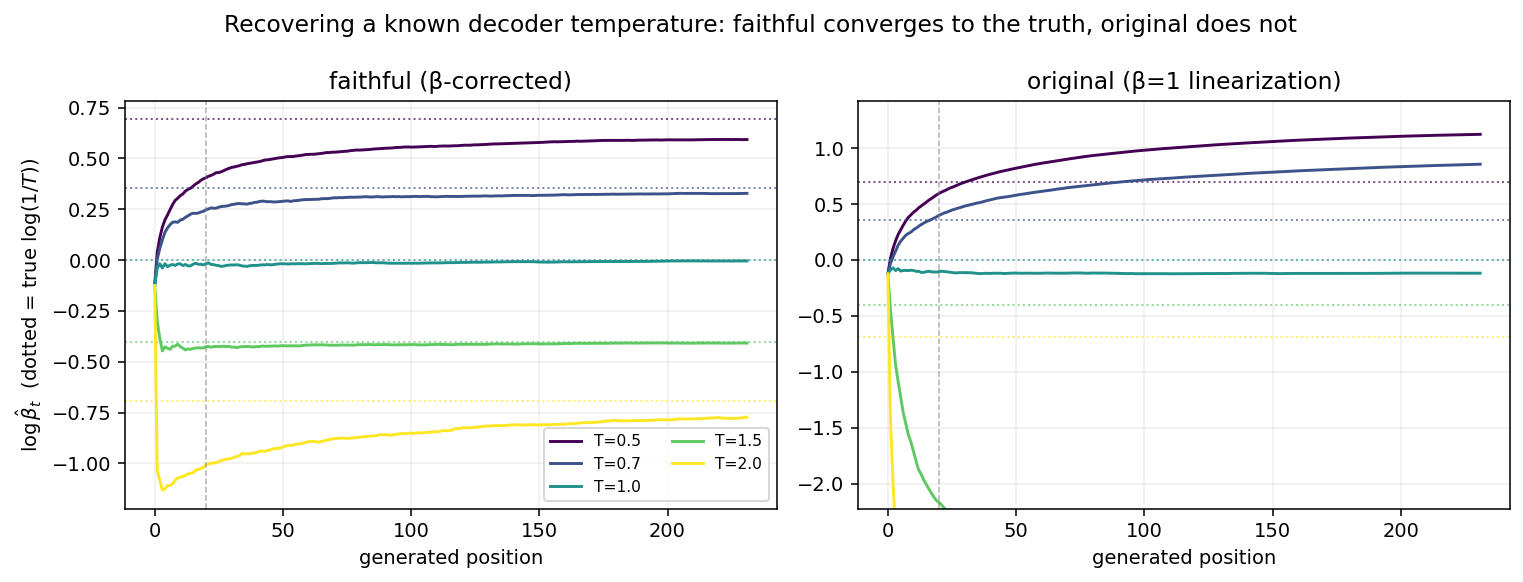
\includegraphics[width=\linewidth]{F_selfcal_recovery.png}
    \column{0.48\textwidth}
      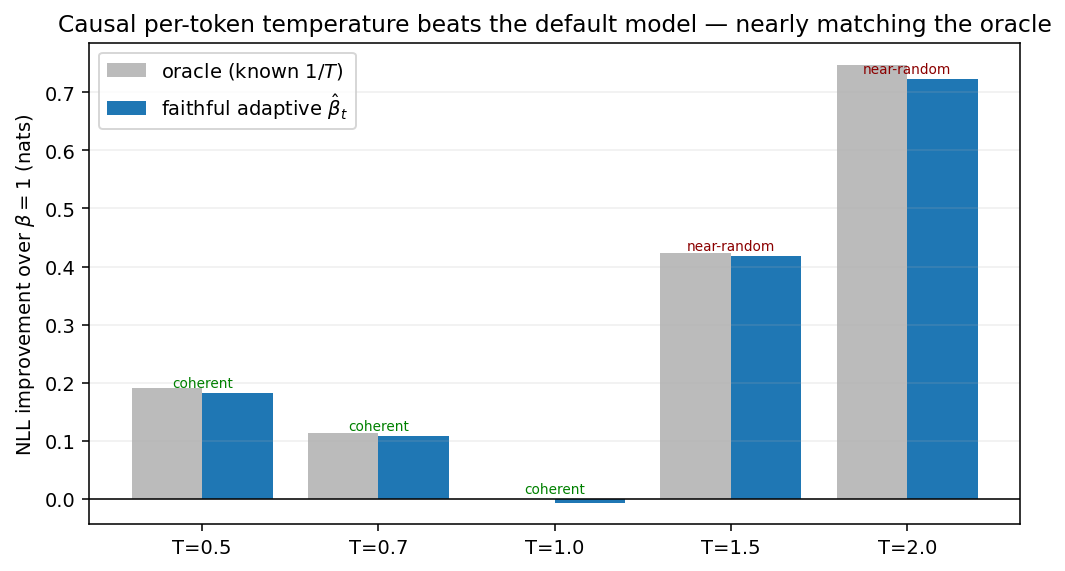
\includegraphics[width=\linewidth]{F_selfcal_nll_gain.png}
  \end{columns}
  \vspace{0.3em}
  \footnotesize
  \begin{itemize}
    \item \textbf{Recovery:} faithful $\hat\beta$ hits the truth (bias
      $\scFaithBiasZeroSeven$ at $T{=}0.7$); the original \emph{diverges}
      ($\scOrigBiasTwo$ at $T{=}2$).
    \item \textbf{Prediction:} the causal per-token temperature beats the default
      $\beta{=}1$ by $\scNllGainZeroSeven$ nats at $T{=}0.7$ (up to $\scNllGainTwo$ at
      $T{=}2$), within $\scOracleGapTwo$ nats of the oracle.
  \end{itemize}
\end{frame}

% ---------------------------------------------------------------------------
\begin{frame}{But does natural text carry a temperature to recover?}
  \begin{center}\footnotesize
    % AUTO-GENERATED by scripts/build_survey_macros.py — do not edit by hand.
\begin{tabular}{lcccc}
\toprule
text type & optimal $T$ & $\Delta$NLL vs $\beta{=}1$ (nats) & $\beta{=}1$ NLL & $H_{\beta=1}$ \\
\midrule
shuffled WikiText & 1.08 & +0.0283$^{**}$ & 7.20 & 6.48 \\
Recam\'an (A005132) & 0.91 & +0.0032$^{**}$ & 0.08 & 0.14 \\
ABC music & 1.03 & +0.0019$^{**}$ & 2.48 & 2.34 \\
WritingPrompts & 1.04 & +0.0011 & 2.87 & 2.74 \\
Telugu & 1.03 & +0.0010$^{**}$ & 1.12 & 1.06 \\
Esperanto & 1.03 & +0.0007 & 2.72 & 2.63 \\
Yoruba & 1.00 & +0.0001 & 3.06 & 3.11 \\
WikiText & 1.00 & -0.0000 & 1.96 & 1.93 \\
Gutenberg (archaic EN) & 1.01 & -0.0001 & 1.87 & 1.85 \\
\bottomrule
\end{tabular}

  \end{center}
  \vspace{0.2em}
  \footnotesize
  \begin{itemize}
    \item \textbf{Qwen is temperature-robust everywhere:} optimal
      $T\in[\scSurvOptTRecaman,\scSurvMaxOptT]$; gains $\le\scSurvGainRecaman$ nats on
      real text ($\scSurvGainShuffledWikitext$ on shuffled gibberish).
    \item \textbf{Recam\'an (A005132)} is the exception: uniquely \emph{under}confident
      ($T=\scSurvOptTRecaman$) --- right so often it should be \emph{sharper}.
      ``Harder $\ne$ mis-temperatured'' (Yoruba is hardest, yet $T\!\approx\!1$).
    \item $\Rightarrow$ no meaningful miscalibration to exploit in the wild.
      \emph{(Checked per-passage on the two worst types: a cross-validated per-passage
      temperature doesn't beat global, and the causal filter captures $\approx0$.)}
  \end{itemize}
\end{frame}

% ---------------------------------------------------------------------------
\begin{frame}{Takeaways}
  \begin{itemize}
    \item The \emph{corrected} filter recovers a decoder temperature from context and
      predicts that text materially better than the default model --- using only the
      model's own logits.
    \item Correct Bayesian bookkeeping (the $\beta,\beta^{2}$ chain-rule terms) is what
      makes it work; the original filter is inconsistent.
    \item Honest scope: an honest \textbf{positive} (Claim 1) \emph{and} an honest
      \textbf{negative} --- natural text is temperature-robust even far out of
      distribution.
  \end{itemize}
\end{frame}

\end{document}
